\documentclass[11pt]{article}

% ---------- Page & Font ----------
\usepackage[margin=2.5cm]{geometry}
\usepackage[utf8]{inputenc}
\usepackage[T1]{fontenc}
\usepackage{lmodern}
\usepackage{microtype}

% ---------- Math & Units ----------
\usepackage{amsmath, amssymb}
\usepackage{siunitx}
\sisetup{per-mode=symbol}

% ---------- Figures & Tables ----------
\usepackage{graphicx}
\usepackage{caption}
\usepackage{subcaption}
\usepackage{float}
\usepackage{booktabs}
\usepackage{array}
\usepackage[table]{xcolor}

% ---------- Code Listings (C, C++, Rust) ----------
\usepackage{listings}
\usepackage{xcolor}

\definecolor{codebg}{RGB}{245,245,245}
\definecolor{codegray}{RGB}{110,110,110}
\definecolor{codeblue}{RGB}{0,80,180}
\definecolor{codegreen}{RGB}{0,120,0}
\definecolor{codered}{RGB}{170,0,0}

\lstdefinelanguage{Rust}{
  keywords={fn, let, mut, pub, struct, enum, impl, trait, for, while, loop, if, else, match, return, use, mod, crate, self, Self, in, as, ref, move, unsafe, dyn, where, const, static, type},
  keywordstyle=\color{codeblue}\bfseries,
  ndkeywords={u8,u16,u32,u64,usize,i8,i16,i32,i64,isize,f32,f64,bool,char,str,String,Vec,Option,Result,Box},
  ndkeywordstyle=\color{codegreen},
  identifierstyle=\color{black},
  sensitive=true,
  comment=[l]{//},
  morecomment=[s]{/*}{*/},
  commentstyle=\color{codegray}\itshape,
  stringstyle=\color{codered},
  morestring=[b]",
}

\lstset{
  backgroundcolor=\color{codebg},
  basicstyle=\ttfamily\footnotesize,
  breaklines=true,
  breakatwhitespace=false,
  frame=single,
  rulecolor=\color{black!20},
  numbers=left,
  numberstyle=\tiny\color{codegray},
  numbersep=8pt,
  showstringspaces=false,
  tabsize=2,
  captionpos=b,
  keywordstyle=\color{codeblue}\bfseries,
  commentstyle=\color{codegray}\itshape,
  stringstyle=\color{codered},
}

% Convenience environments per language
\lstnewenvironment{ccode}[1][]{\lstset{language=C,#1}}{}
\lstnewenvironment{cppcode}[1][]{\lstset{language=C++,#1}}{}
\lstnewenvironment{rustcode}[1][]{\lstset{language=Rust,#1}}{}

% ---------- Misc ----------
\usepackage{hyperref}
\hypersetup{colorlinks=true, linkcolor=blue, citecolor=blue, urlcolor=blue}
\usepackage{enumitem}
\usepackage{xurl}

% ---------- Custom colored boxes for special sections ----------
\usepackage[most]{tcolorbox}

\newtcolorbox{hypothesisbox}{
  colback=blue!4, colframe=blue!50!black, title=Pre-Experiment Hypothesis,
  fonttitle=\bfseries, breakable
}
\newtcolorbox{failurebox}{
  colback=red!4, colframe=red!50!black, title=Negative / Failure Case,
  fonttitle=\bfseries, breakable
}
\newtcolorbox{anomalybox}{
  colback=yellow!8, colframe=orange!70!black, title=Honest Anomalies,
  fonttitle=\bfseries, breakable
}

% ---------- Title Info ----------
\title{\textbf{ECSE-6320 Advanced Computer Systems \\ Project 3 Report}}
\author{Cooper Werner \\\small Rensselaer Polytechnic Institute \\ \small wernec6@rpi.edu }
\date{\today}

\begin{document}

\maketitle

\tableofcontents
\newpage

% =====================================================
\section{Introduction}
% Context, motivation, system under test, and objective of this experiment.

% =====================================================

The goal of this project is to analyze how block size, access pattern, read/write ratio, queue depth, data pattern, and
device state impact SSD performance. I utilized the FIO utility to run tests on my secondary SSD, and I report my
findings below.

\section{Pre-Experiment Hypotheses}

\begin{hypothesisbox}
	\textbf{Hypothesis:} \\
	% State the falsifiable prediction before running anything.

	I think that in general, SSD writes will be slower than reads utilizing the same block size, access pattern, and queue
	depth.

	\textbf{Reasoning:} \\
	% Why do you expect this outcome? Reference architecture, prior results, theory.
	From my prior experience installing software and copying files, I have observed that writing to an SSD is slower than
	reading from it. So I would expect that this would be the case in general.

	\textbf{Predicted quantitative outcome:} \\
	\begin{center}
		\captionof{table}{Predicted Read vs Write Speed for Various Block Sizes}
		\label{tab:hypothesis-huge-pages}
		\begin{tabular}{lcc}
			\toprule
			\textbf{Block Size} & \textbf{Read Speed} & \textbf{Write Speed} \\
			\midrule
			4 KiB               & 500 MB/s            & 400 MB/s             \\
			16 KiB              & 600 MB/s            & 500 MB/s             \\
			32 KiB              & 700 MB/s            & 600 MB/s             \\
			64 KiB              & 800 MB/s            & 700 MB/s             \\
			128 KiB             & 900 MB/s            & 800 MB/s             \\
			256 KiB             & 1000 MB/s           & 900 MB/s             \\
			512 KiB             & 1100 MB/s           & 1000 MB/s            \\
			\bottomrule
		\end{tabular}
	\end{center}
\end{hypothesisbox}

\begin{hypothesisbox}
	\textbf{Hypothesis:} \\
	% State the falsifiable prediction before running anything.

	Accessing data with in a sequential pattern will be faster than accessing data with a random pattern, given the same
	block size and queue depth.

	\textbf{Reasoning:} \\
	% Why do you expect this outcome? Reference architecture, prior results, theory.

	Sequential access patterns allow the SSD to optimize its internal operations, such as read-ahead and write buffering,
	leading to better performance compared to random access patterns. It will also reduce the number of seek operations and
	improve cache utilization, resulting in lower latency and higher throughput.

	\textbf{Predicted quantitative outcome:} \\
	% e.g., "Expect L2 miss rate to decrease by \SI{15}{\percent} \pm \SI{3}{\percent}"
	\begin{center}
		\captionof{table}{Predicted Slowdown for Sequential vs Random Access}
		\label{tab:hypothesis-simd}
		\begin{tabular}{lccc}
			\toprule
			\textbf{Access Pattern} & \textbf{Slowdown For Read} & \textbf{ Slowdown For Write} \\
			\midrule
			Sequential              & 1.0x                       & 1.0x                         \\
			Random                  & 1.5x                       & 1.5x                         \\
			\bottomrule
		\end{tabular}
	\end{center}
\end{hypothesisbox}

% =====================================================
\section{Measurement Discipline}
% Describe methodology: isolation (core pinning, turbo/frequency scaling disabled, etc.),
% number of trials, warm-up runs, statistical treatment (mean/median/stdev/CI),
% timer resolution, environmental controls.

To collect the data I utilized AI to help me write a shell script tha ran a variety of FIO commands to collect data
about my SSD's performance. To ensure the safety of my data, I ensured that the script required the user to enter the
specific drive they are profiling, the script will refuse to run if the drive has a root or boot directory on it. Then
the user has to confirm execution before testing on the drive will start.

\subsection{Experimental Setup}
\begin{itemize}[leftmargin=1.5em]
	\item \textbf{Hardware:} CPU: x86\_64 AMD Ryzen AI 7 350 w/ Radeon 860M, Memory: 32GB LPDDR5 @ 5600MT/s, SSD: OEM Samsung SSD 980 Pro 1TB NVMe PCIe Gen4
	\item \textbf{OS / Kernel:} Pop\_OS! 24.04 Running Linux 7.0.11-76070011-generic
	\item \textbf{FIO Version:} fio-3.36
	\item \textbf{Isolation techniques:} Tested on dedicated drive with no other processes running, CPU frequency scaling disabled, and CPU pinned to a single core.
	\item \textbf{GB Written Per Trial:} 10 GB for each test to ensure steady-state performance.
\end{itemize}

The computer was restarted before the test to ensure that the SSD was in a known state, the comptuer was idle, and no
other processes were running. The computer was plugged in and running on AC power to avoid any performance throttling
due to battery saving features. Lastly, the CPU govenor was set to performance mode to avoid any frequency scaling
during the tests.

\subsection{Statistical Treatment}

Due to the large number of experiments and the time required to run each one, I only ran each test once. However, I
ensured that each test was run for a sufficient duration (10 GB of data written) to reach steady-state performance,
minimizing the impact of transient effects on the results.

\section{Results}

\subsection{Bandwidth vs Latency for Various Queue Depths}
\begin{figure}[H]
	\centering
	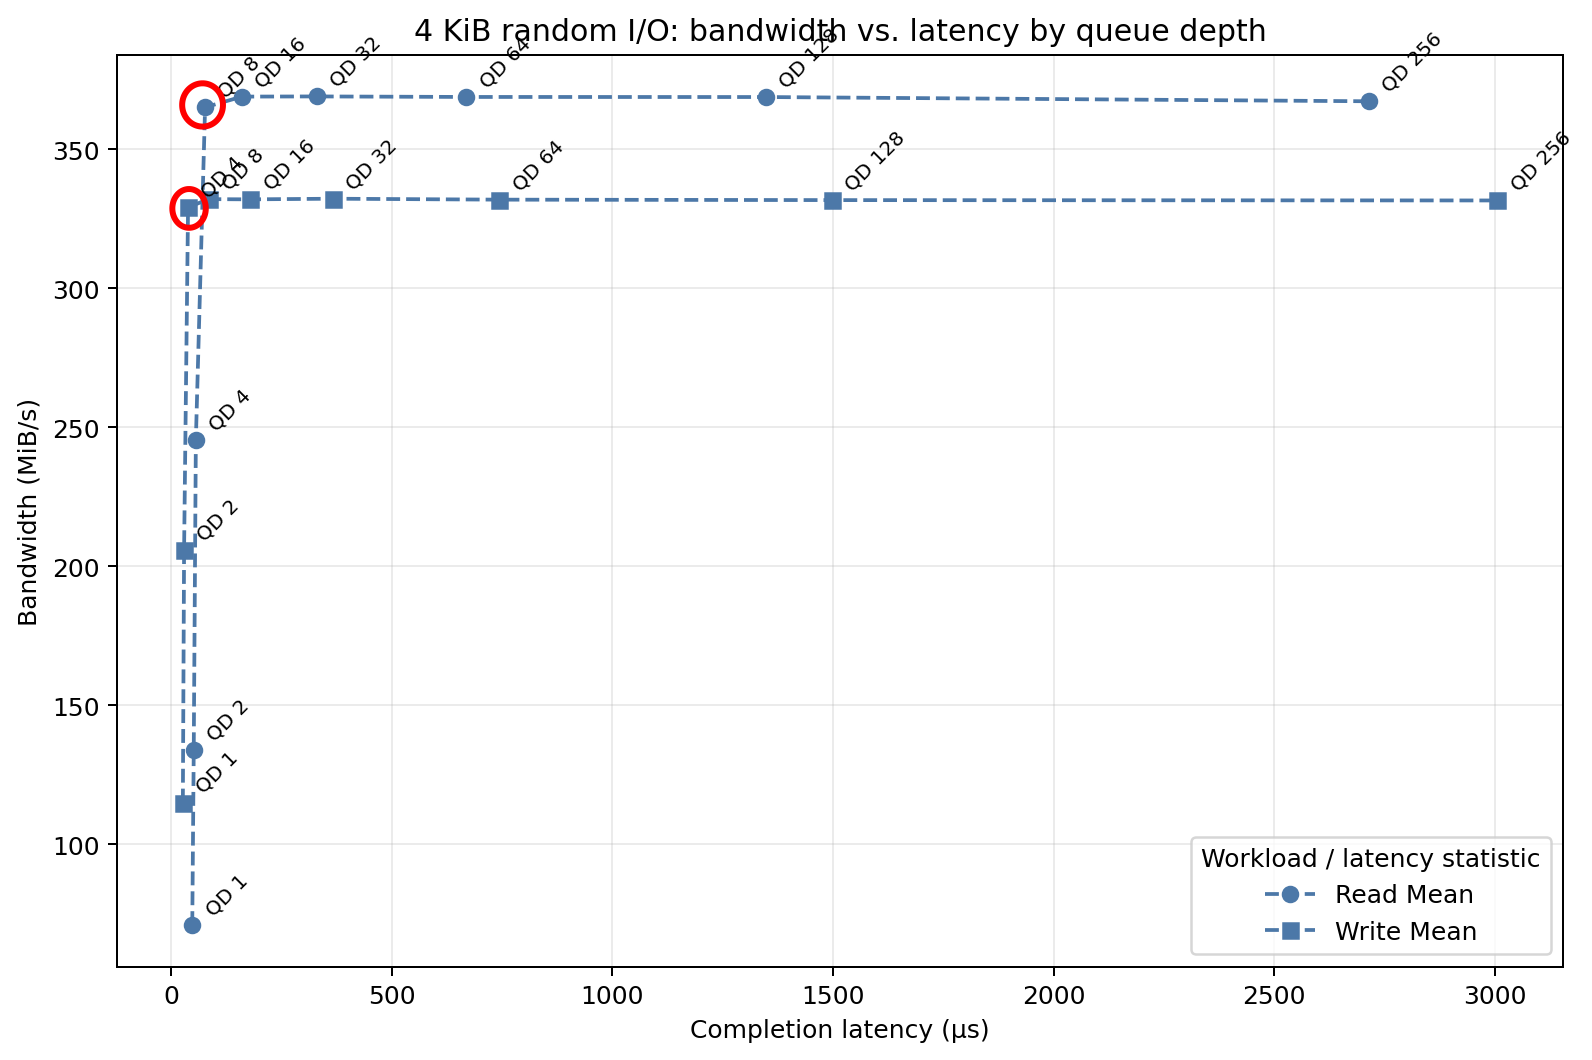
\includegraphics[width=0.85\textwidth]{../analysis/plots/queue_depth_bandwidth_vs_latency.png}
	\caption{Plot of bandwidth vs latency for various queue depths. At a queue depth around 4 or 8, bandwidth capacity increases significantly, and the
		latency of each request starts to increase rapidly. }
	\label{fig:bandwidth-vs-latency-queue-depth}
\end{figure}

Figure \ref{fig:bandwidth-vs-latency-queue-depth}demonstrates that SSDs can optimize for bandwidth or latency using
request queuing. Having a greater queue depth means that the SSD can best utilize the PCIe bus for transfering data
to/from RAM. This queuing comes with a tradeoff for latency, as queue depth grows, latency also does as predicted by
Little's Law: $L = \lambda R$. Increasing the queue depth increases the number of outstanding requests, $L$, and since
$\lambda$ is a constant, the latency for each individual request must increase too.

\subsection{Zero-Queue Baseline Latency and Bandwidth}

\begin{table}[H]
	\centering
	\caption{Zero-Queue Baseline Latency and Bandwidth}
	\label{tab:zero-queue-baseline}
	\begin{tabular}{@{}lcccc@{}}
		\toprule
		Setup                   & Mean BW (MB/s) & P95 Lat. ($\mu s$) & P99 Lat. ($\mu s$) & P99.9 Lat. ($\mu s$) \\
		\midrule
		4KiB Random Read        & 67.9           & 63.7               & 74.4               & 150.5                \\
		4KiB Random Write       & 118.2          & 37.1               & 43.3               & 81.4                 \\
		128KiB Sequential Read  & 1,490.7        & 116.2              & 144.4              & 199.7                \\
		128KiB Sequential Write & 1,755.7        & 82.4               & 119.3              & 173.1                \\
		\bottomrule
	\end{tabular}
\end{table}

The zero-queue baseline latency and bandwidth data from table \ref{tab:zero-queue-baseline} show an interesting pattern
that shows up a few times in the data, the write bandwidth is larger than the read bandwidth and the write latency is
lower than the read bandwidth. This is true for both access patterns and block sizes for the baseline. This contradicts
my hypothesis from above.

\subsection{Near-Knee Tail Latency Characterization}

\begin{table}[H]
	\centering
	\caption{Near-Knee Tail Read Latency Characterization}
	\label{tab:near-knee-read}
	\begin{tabular}{@{}lcccc@{}}
		\toprule
		Queue Depth & P95 Lat. ($\mu s$) & P99 Lat. ($\mu s$) & P99.9 Lat. ($\mu s$) \\
		\midrule
		QD4         & 82.4               & 100.8              & 130.6                \\
		QD8         & 105.9              & 128.5              & 152.5                \\
		QD16        & 181.2              & 203.8              & 236.5                \\
		\bottomrule
	\end{tabular}
\end{table}

\begin{table}[H]
	\centering
	\caption{Near-Knee Tail Write Latency Characterization}
	\label{tab:near-knee-write}
	\begin{tabular}{@{}lcccc@{}}
		\toprule
		Queue Depth & P95 Lat. ($\mu s$) & P99 Lat. ($\mu s$) & P99.9 Lat. ($\mu s$) \\
		\midrule
		QD4         & 55.0               & 70.1               & 85.5                 \\
		QD8         & 107.0              & 130.5              & 152.6                \\
		QD16        & 214.0              & 220.1              & 276.5                \\
		\bottomrule
	\end{tabular}
\end{table}

As seen in Figure \ref{fig:bandwidth-vs-latency-queue-depth} the knee queue depth for read is a queue depth of 8, for
write the knee is at a queue depth of 4. By looking at the tail latencies, for read, having a queue depth of 4 does not
significantly decrease the latency of each request while significantly impacting the maximum bandwidth.

\subsection{Block Size Sweep}
\subsubsection{Random Read / Write}

\begin{figure}[H]
	\centering
	\begin{subfigure}[b]{0.48\textwidth}
		\centering
		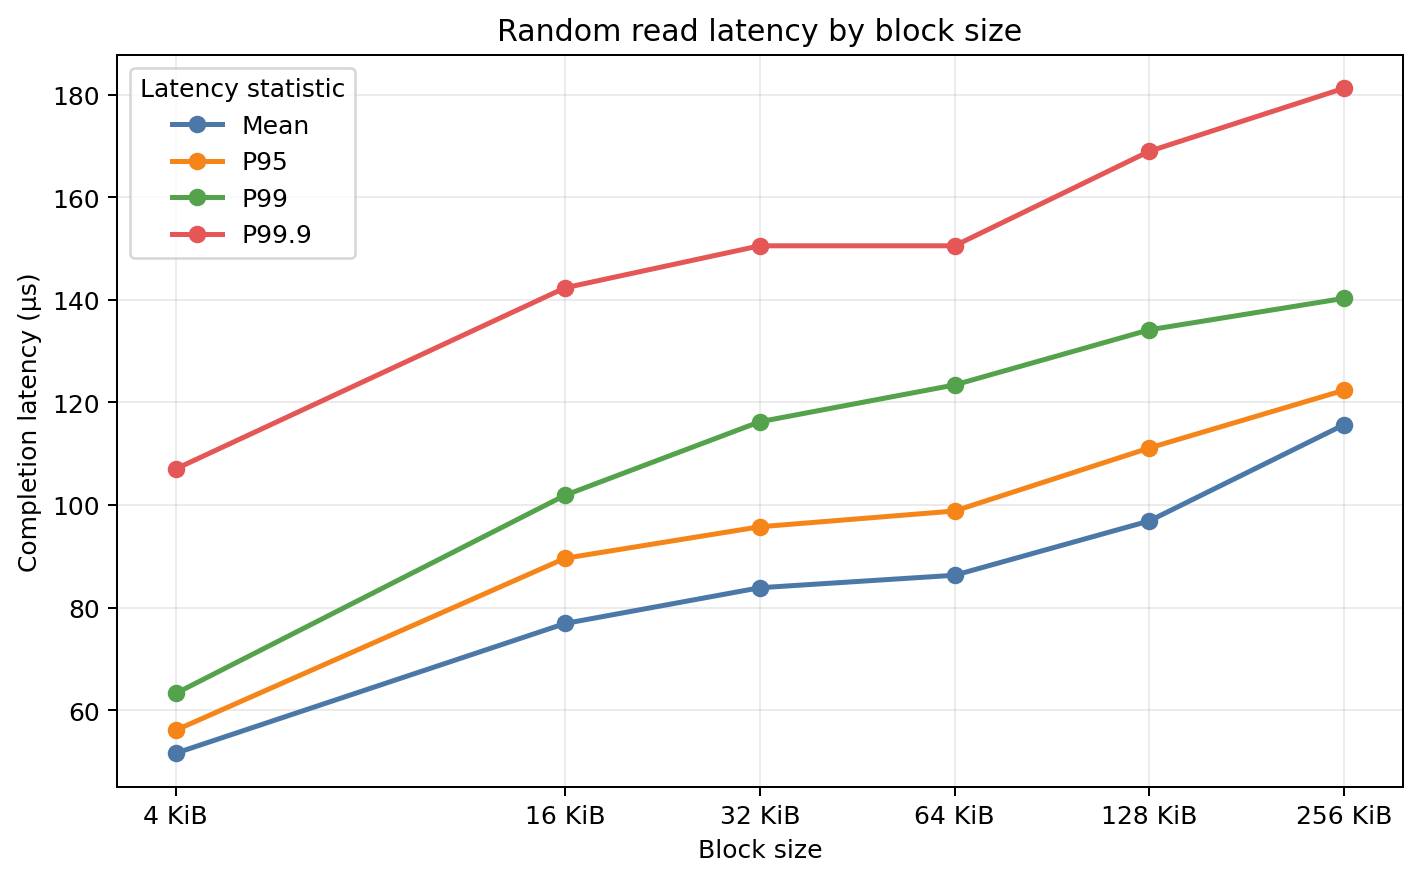
\includegraphics[width=\textwidth]{../analysis/plots/block_size_randread.png}
		\caption{Plot of SSD random read latencies for different sized blocks with a fixed queue depth of 1.}
		\label{fig:block-size-randread}
	\end{subfigure}
	\hfill
	\begin{subfigure}[b]{0.48\textwidth}
		\centering
		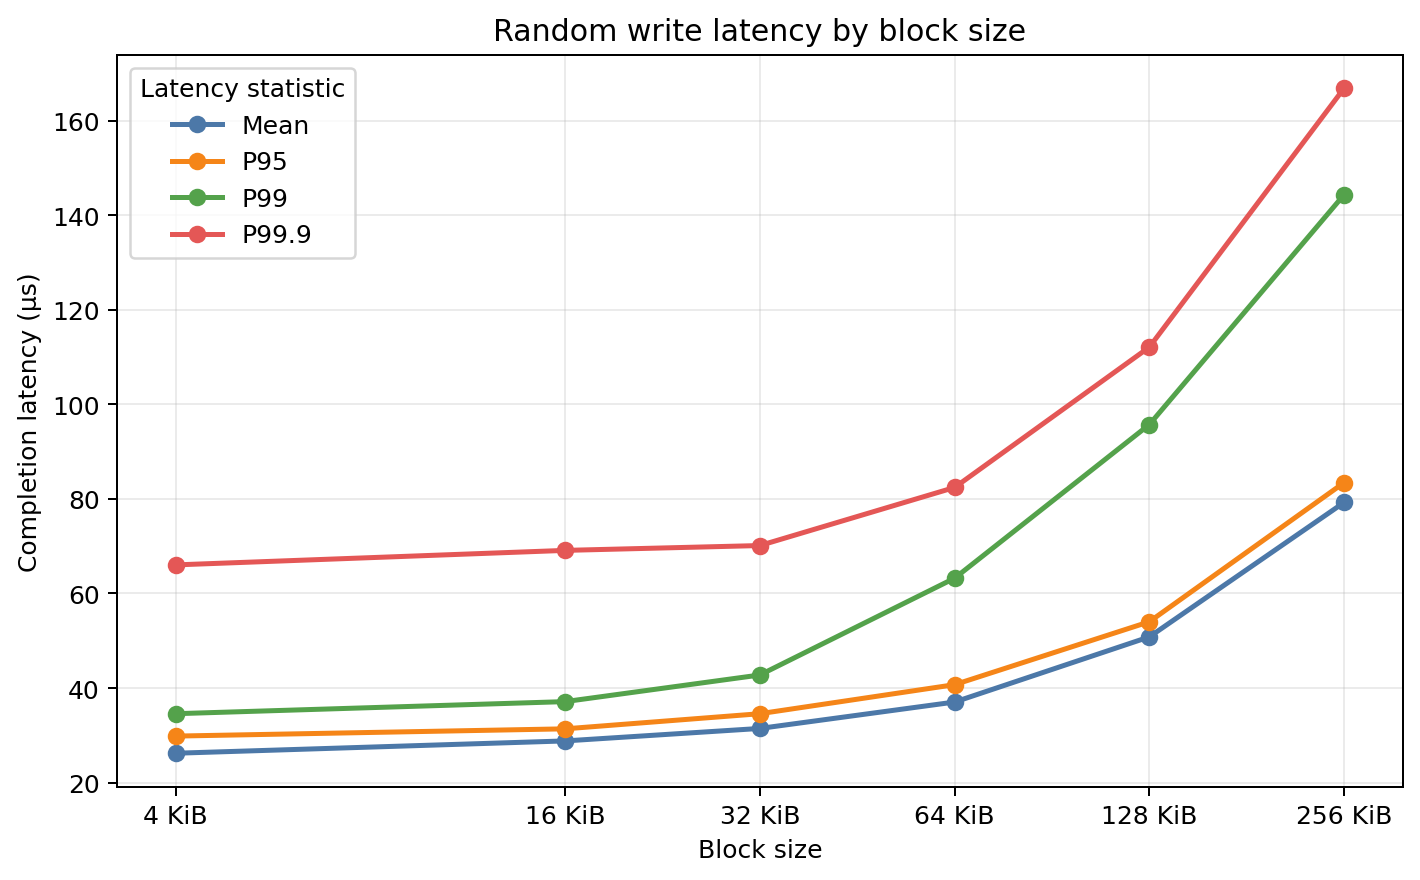
\includegraphics[width=\textwidth]{../analysis/plots/block_size_randwrite.png}
		\caption{Plot of SSD random write latencies for different sized blocks with a fixed queue depth of 1.}
		\label{fig:block-size-randwrite}
	\end{subfigure}
	\caption{Side-by-side comparison of \dots}
	\label{fig:block-sweep-both-random}
\end{figure}

\subsubsection{Sequential Read / Write}

\begin{figure}[H]
	\centering
	\begin{subfigure}[b]{0.48\textwidth}
		\centering
		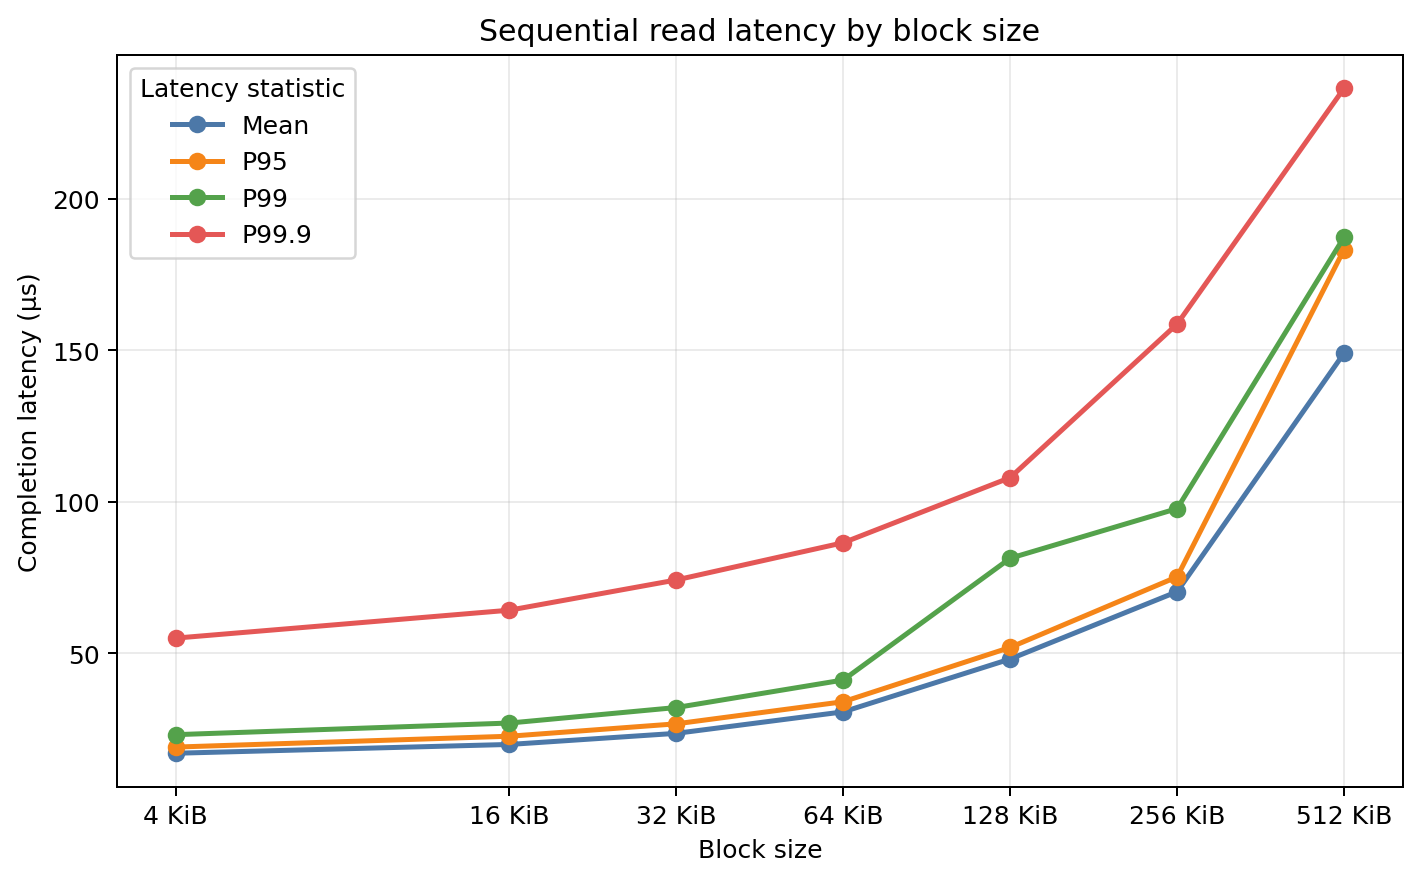
\includegraphics[width=\textwidth]{../analysis/plots/block_size_read.png}
		\caption{Plot of SSD sequential read latencies for different sized blocks with a fixed queue depth of 1.}
		\label{fig:block-size-sequential-read}
	\end{subfigure}
	\hfill
	\begin{subfigure}[b]{0.48\textwidth}
		\centering
		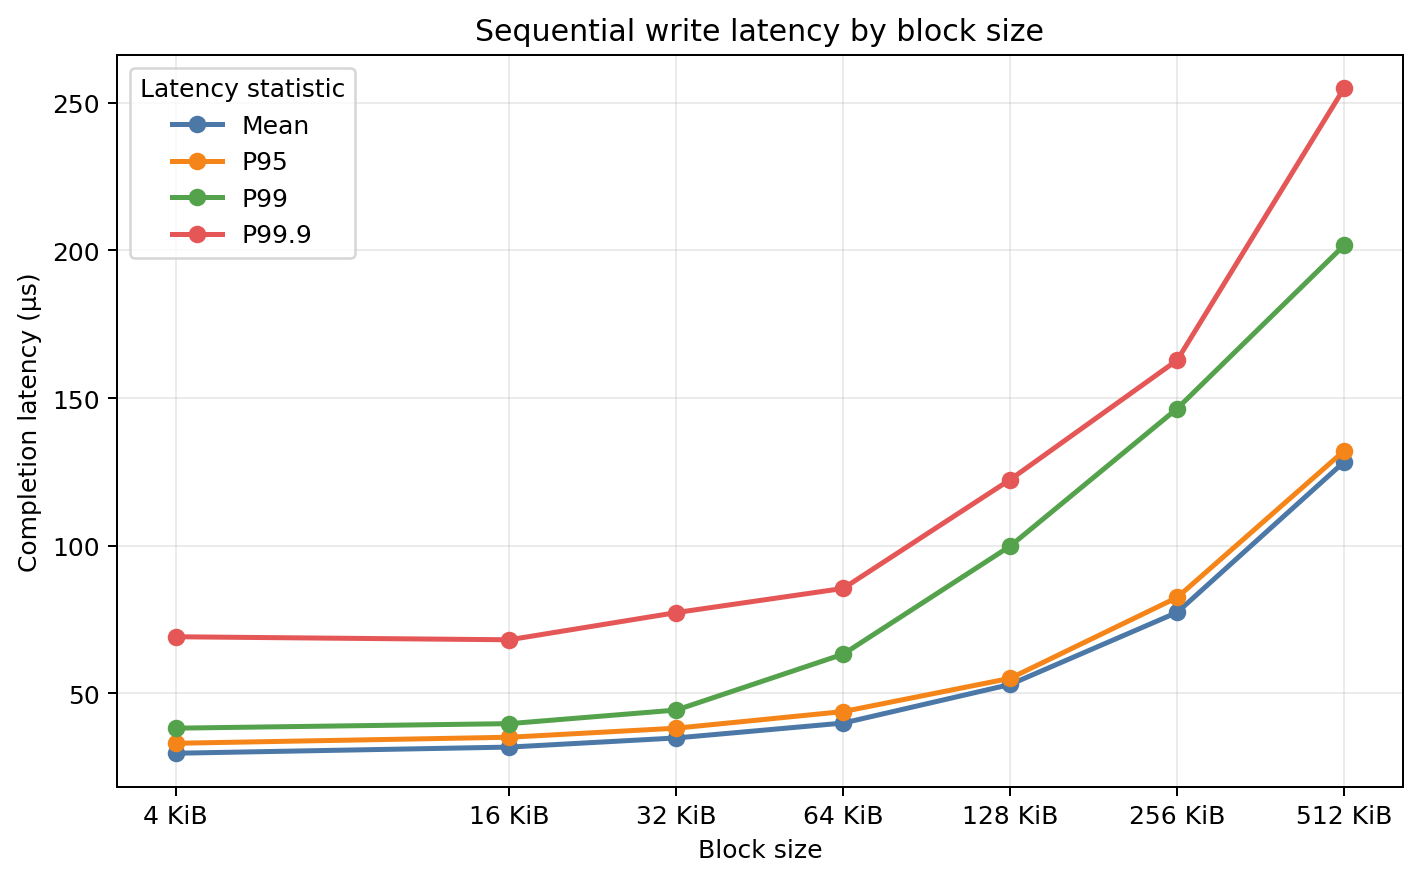
\includegraphics[width=\textwidth]{../analysis/plots/block_size_write.png}
		\caption{Plot of SSD sequential write latencies for different sized blocks with a fixed queue depth of 1.}
		\label{fig:block-size-sequential-write}
	\end{subfigure}
	\caption{Side-by-side comparison of \dots}
	\label{fig:block-sweep-both-sequential}
\end{figure}

\begin{figure}[H]
	\centering
	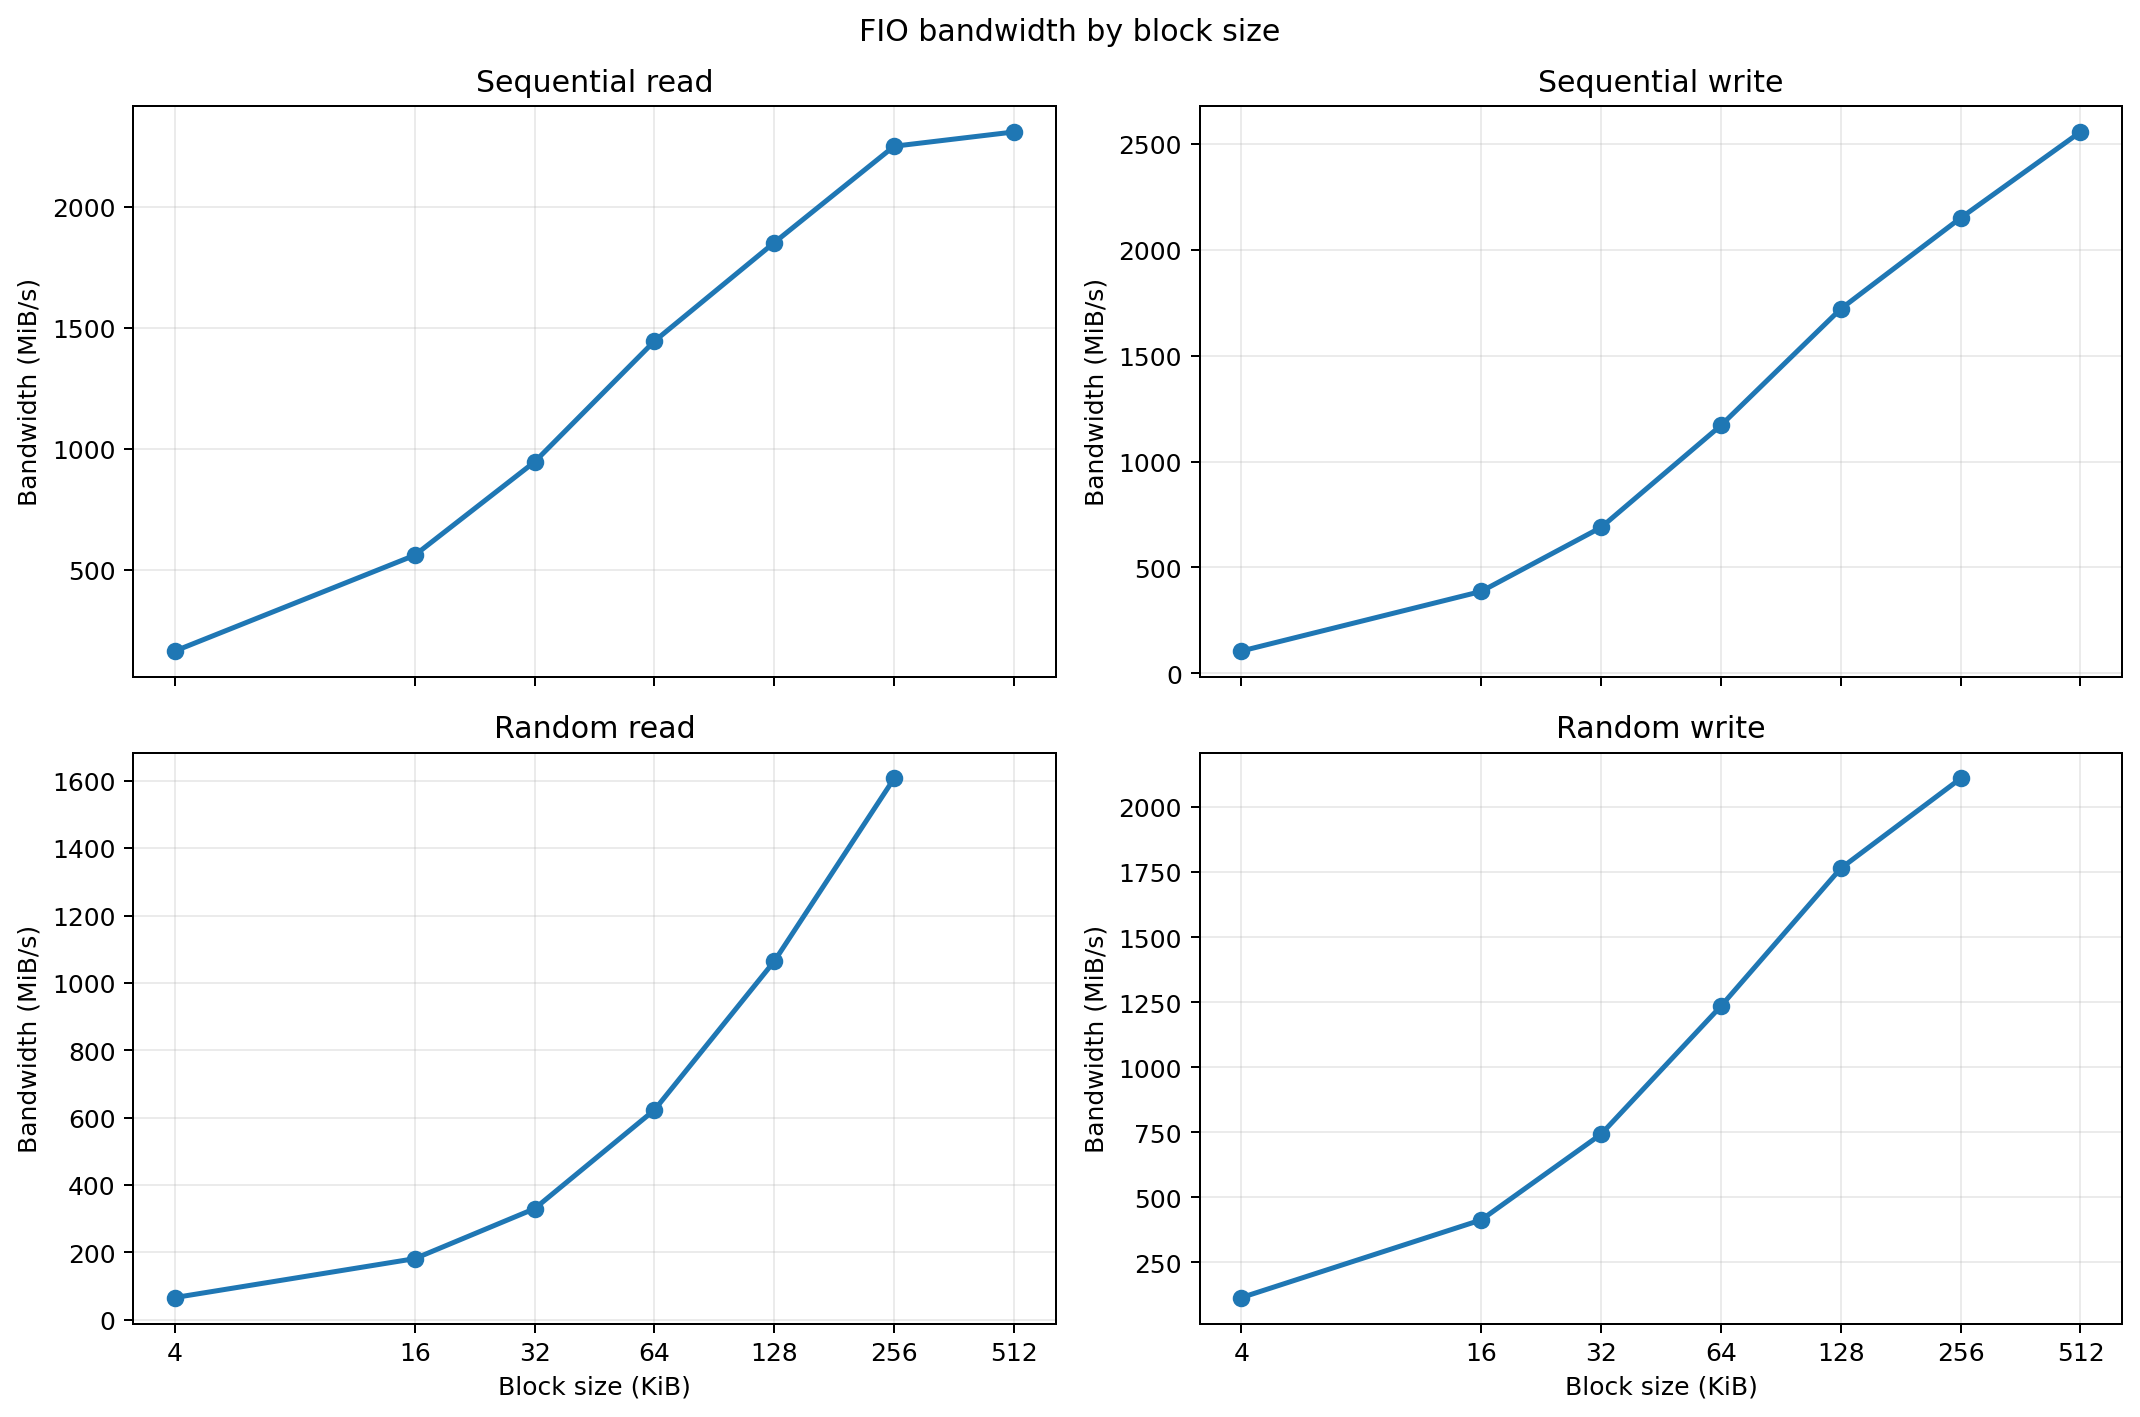
\includegraphics[width=0.85\textwidth]{../analysis/plots/block_size_bandwidth.png}
	\caption{Plots of bandwidth as block size changes with a fixed queue depth of 1.}
	\label{fig:block-size-bandwidth}
\end{figure}

Changing the size of the blocks has a very similar effect to changing the queue depth. As you increase block size, the
SSD is able to batch requests and read / write more to the NAND flash cells. However this comes at the cost of latency,
larger blocks take more time to write to the drive and therefore will have larger latencies.

\subsection{Read / Write Mix Sweep}

\begin{figure}[H]
	\centering
	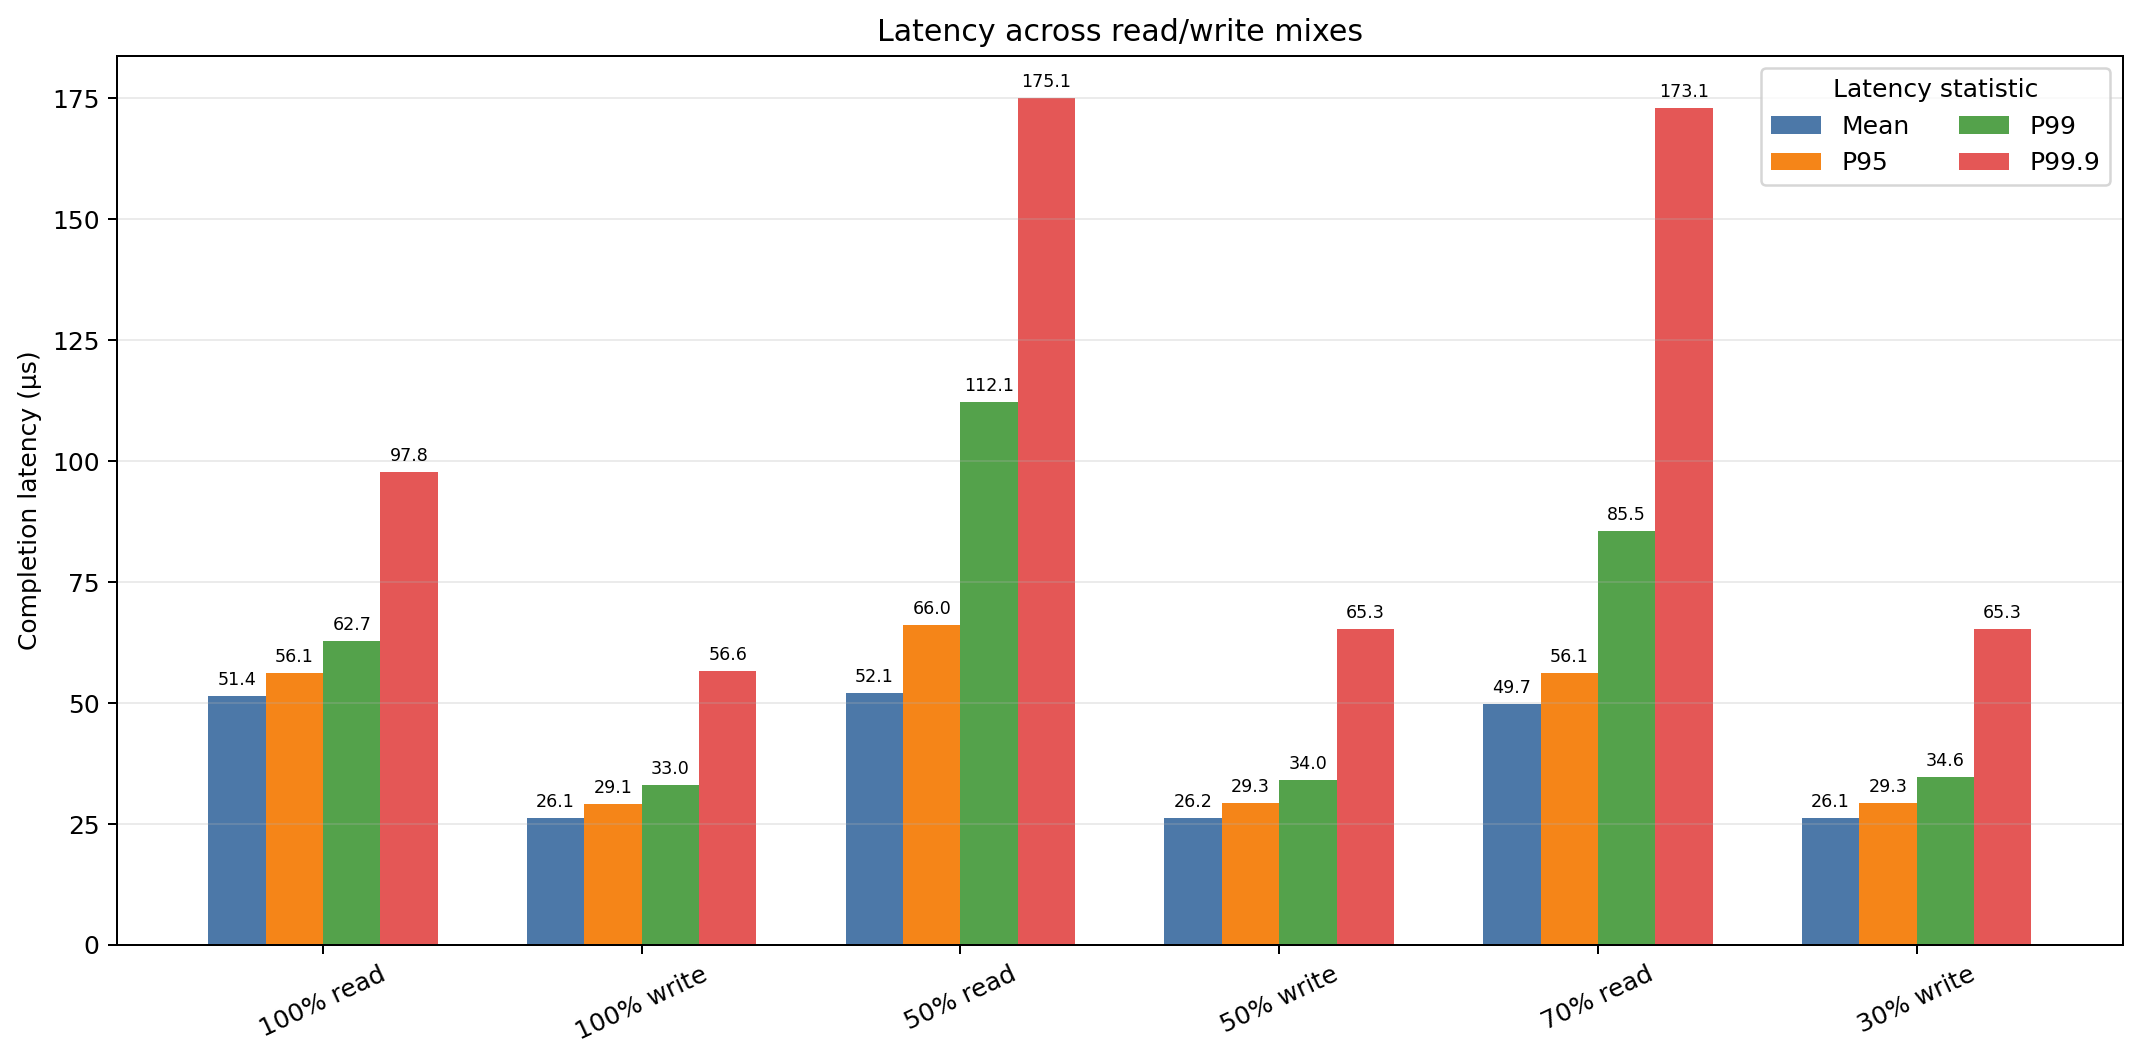
\includegraphics[width=0.85\textwidth]{../analysis/plots/read_write_mix_latency.png}
	\caption{Bar chart showing the average, P95, P99, and P99.9 latencies for read and write operations for the different mixes. The mixes
		tested were 100\% read, 100\% write, 50/50\% read-write, 70\%/30\% read-write.}
	\label{fig:read-write-mix-latency}
\end{figure}

The read operations had latencies that were consistently higher than the write latencies. In the mixes with 50\% or
70\% reads the P99 and P99.9 latencies for the read operations specifically increased far past the mix where reads were
100\% of the operations. This did not happen for the write operations which had consistent latencies for each of the
mixes. This may be due to the SLC write cache helping to cache write requests while reads are in progress, but the read
operations have to be blocked if a write operation is happening at the same time since data served must be up to date.

\subsection{Impact of Data Compressibility On Latency}

\begin{figure}[H]
	\centering
	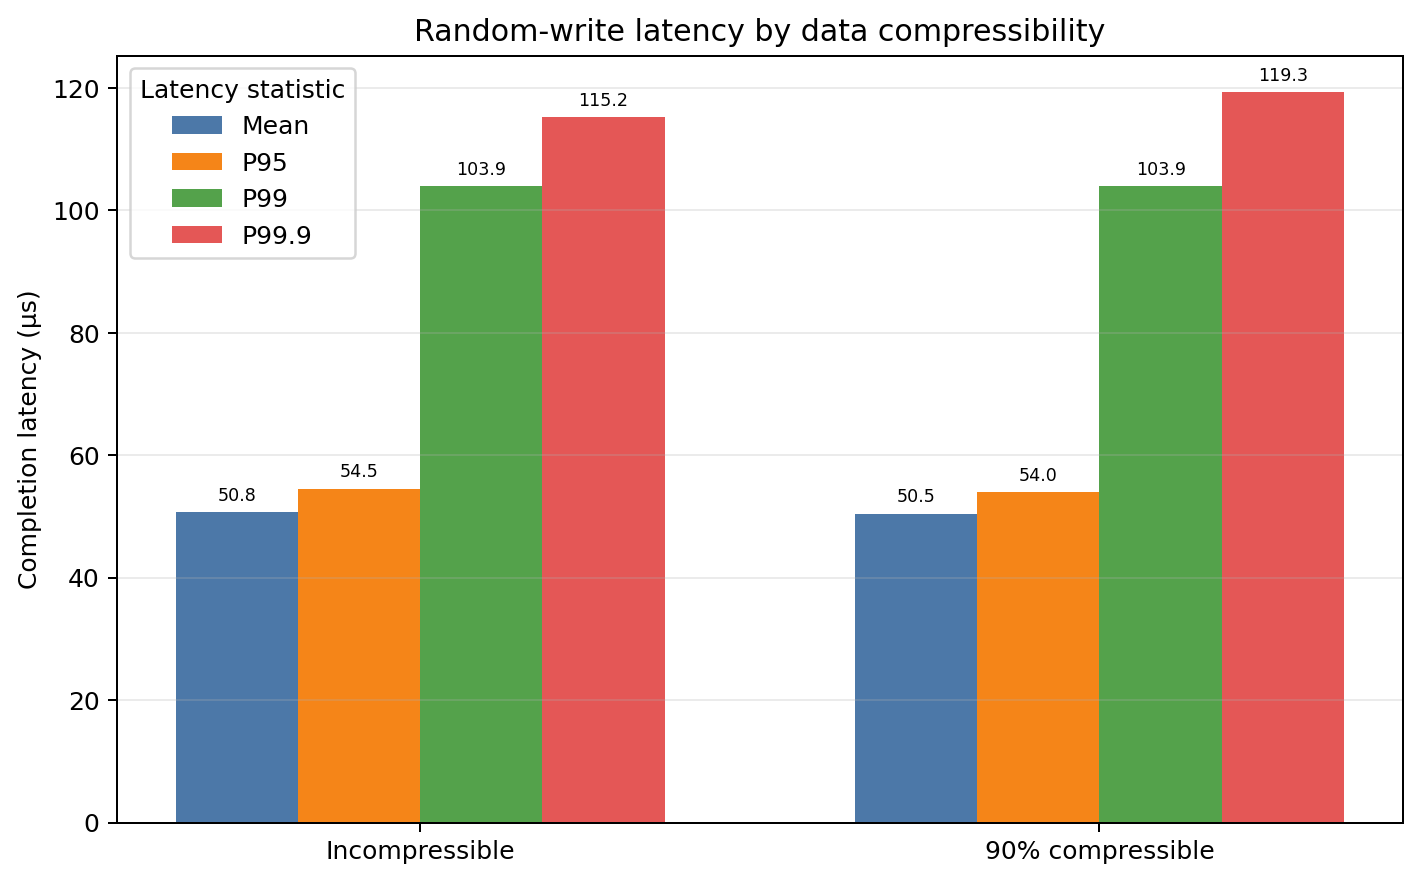
\includegraphics[width=0.85\textwidth]{../analysis/plots/data_compressibility_latency.png}
	\caption{Bar chart showing latencies for saving incompressible data and highly compressible data.}
	\label{fig:data-compressibility-latency}
\end{figure}

There was no significant difference in lattency for saving compressible vs incompressible data. This is because the SSD
tested, the SAMSUNG MZVL21T0HCLR, lacks a hardware-level data compression function in the SSD controller. This means
that regardless of data compressibility, the same amount of data is written to disk and the latencies remain the same.
\cite{Chiappetta2020Samsung}\cite{Klaus2022Samsung}

\subsection{Impacts of SSD State on Latency and Bandwidth}

\begin{table}[H]
	\centering
	\caption{Impacts of SSD State on Write Latency and Bandwidth}
	\label{tab:ssd-state-latency-bandwidth}
	\begin{tabular}{@{}lcccc@{}}
		\toprule
		SSD State                   & Mean BW (MB/s) & P95 Lat. ($\mu s$) & P99 Lat. ($\mu s$) & P99.9 Lat. ($\mu s$) \\
		\midrule
		Fresh First Write           & 1,748.7        & 57.6               & 99.8               & 124.4                \\
		Garbage Collection Stress   & 314.7          & 432.1              & 1,581.1            & 2,736.1              \\
		Garbage Collection Recovery & 327.6          & 415.7              & 1,028.1            & 2,039.8              \\
		Steady State                & 3,232.2        & 2,146.3            & 3,915.8            & 6,651.9              \\
		SLC Cache Exhaustion        & 3,473.3        & 7,634.9            & 8,454.1            & 13,434.9             \\
		\bottomrule
	\end{tabular}
\end{table}

Table \ref{tab:ssd-state-latency-bandwidth} demonstrates the variablility in SSD performance depending on SSD state.
When the SSD is fresh, it is able to maintain a high write bandwidth with low latencies. As the SSD fills up and the
garbage collector starts running the maximum write bandwidth decreases significantly and latencies start increasing. In
steady-state the drive has an impressive write bandwidth, but its latencies can increase to close to 6ms for a single
request. This is amplified when the SLC cache is exhausted, cache exhaustion increases the P99.9 latencies to over
13ms.

\section{Negative / Failure Case}

\begin{failurebox}
	\textbf{Experimental Pitfall:} \\

	My script runs the FIO commands immediately after the termination of the previous one without providing the SSD time to
	rest, handle garbage collection, or cool down. This could create confounding results in the different experiments. I
	also don't have good data on the SSD temperature during the experimental runs. Lastly, my SSD lives in a laptop chassis
	which does not provide an optimal path for heat dissipation. \\

	\textbf{How would I fix this?} \\

	If I were to continue looking at this I would change the experimental setup to give the SSD time to return to restful
	state between each run. I would also move testing from my laptop to a desktop tower or open-air testbench to remove the
	impacts of thermal effects.

\end{failurebox}

% =====================================================
\section{Discussion}

My first hypothesis was disproven by the data I collected. Consistently, the write operations had higher bandwidths and
lower latencies than read operations of the same queue depth, block size, and access pattern. This is a bit perplexing
to me give my experience installing software and copying files between disks in the past where read operations feel
faster than write operations. Perhaps this is due to the SLC cache helping to make writes more efficicent and that my
test file size was not large enough to fully exhaust the cache. It would be interesting to look into this further.

My second hypothesis was mostly correct, but the slowdown was not as extreme as I had predicted it to be. Random reads
had a 1.43x decrease in bandwidth, but only a 1.09x increase in latency. The general idea was correct, but my predicted
magnitude was off by a bit.

I noticed that for the bandwidth vs block size plots, the trend indicated that increasing the block size futher would
be able to increase bandwidth further. It would be interesting to explore this further and look at which queue depths
and block sizes maximize bandwidth or minimize latency.

\section{Conclusion}

SSD Performance is strongly dependent on block size, access pattern, queue depth, and device state. If latency or
bandwidth is important for the application, programmers should carefully balance block size, queue depth, and access
pattern to ensure that SSD characteristics match the required spec for the application.

\appendix

\section{AI Usage}

AI helped me write the code required for the experiment, it helped develop scripts for running all the required
experiments, assisted in developing python code to create plots and figures. Lastly, I utilized AI in developing the
experimental design and troubleshooting anomalies in the data.

\begin{enumerate}
	\item Helped me determine the best way to perform this experiment:
	      https://claude.ai/share/64d5d392-8521-4067-9c41-80704ce5ede0
\end{enumerate}

I also made extensive use of OpenCode (an open source coding agent) to develop scripts, experiment code, and plotting
code. I reveiewed all output for correctness and accuracy. Making minor fixes where applicable. Transcripts for the
OpenCode sessions are available in \texttt{./OpenCode}

\section{Additional Data / Raw Logs}
% Optional: full result dumps, extra plots, raw perf output, etc.
Raw data can be found \texttt{./fio-results-20261016-200949}. Plots and plotting code can be \texttt{./analysis}.

\bibliographystyle{IEEEtran}     % Sets the style to IEEE
\bibliography{references}

\end{document}